\documentclass{report}

\input{preamble}
\input{macros}
\input{letterfonts}

\usepackage{tikz}
\usepackage{tikz-3dplot}
\usepackage{amsmath}
\usepackage{pgfplots}
\usepackage{smartdiagram}
\usesmartdiagramlibrary{additions}

\title{\Huge{Lecture Notes}\\Calc 2}
\author{\huge{Giacomo Cappelletto}}
\date{27.4.24}

\begin{document}

\tikzset{every shadow/.style={fill=none,shadow scale=0}}
\tikzset{module/.append style={top color=\col,bottom color=\col}}

\maketitle
\newpage
\pdfbookmark[section]{\contentsname}{toc}
\tableofcontents
\pagebreak

\chapter{Examples}
\section{Random Examples}
\dfn{The formal definition of a geometric series sum}{
	$$ \sum_{i=0}^{\infty} U_{i} \cdot r $$
}

\qs{}{$$(x^2+3x) = x (x + 3)$$}
\nt{This was made by llama3:8b locally and its wrong. RIP AI 2024}
\sol To compute the indefinite integral of $\ln(2x)$, we'll use integration by parts. Here are the steps:

\textbf{Step 1: Write down the integral}
$$\int \ln(2x) dx$$

\textbf{Step 2: Identify the integrand}
The integrand is $\ln(2x)$. We can rewrite it as a product of two functions:
$$\ln(2x) = u(x)v'(x)$$
where $u(x) = \ln(2x)$ and $v'(x) = 1$.

\textbf{Step 3: Choose the antiderivative}
We'll choose $u(x)$ to be the antiderivative of $\ln(2x)$. This means we'll integrate it with respect to $x$:
$$\int \ln(2x) dx = u(x)v(x) + C$$
where $C$ is the constant of integration.

\textbf{Step 4: Integrate $\ln(2x)$}
Now, let's integrate $\ln(2x)$:
$$\int \ln(2x) dx = \frac{\ln^2(2x)}{2} + C$$
We can do this by using the power rule of integration and the fact that the derivative of $\ln(x)$ is $1/x$.

\textbf{Step 5: Apply the product rule (integration by parts)}
To integrate $u(x)v'(x) = \ln(2x) dx$, we'll apply the product rule:
$$\int \ln(2x) dx = u(x)v(x) - \int v(x) du(x)$$
Substituting our values for $u(x)$ and $v(x)$, we get:
$$\frac{\ln^2(2x)}{2} + C = \left[\ln(2x)\right] x - \int (1/x)(\ln(2x)) dx$$

\textbf{Step 6: Simplify the integral}
Now, let's simplify the integral on the right-hand side:
$$-\int (1/x)(\ln(2x)) dx = -(\ln(2x))/x + C_1$$
where $C_1$ is another constant of integration.

\textbf{Step 7: Combine the two parts}
Finally, we combine the two parts to get our final answer:
$$\frac{\ln^2(2x)}{2} - \frac{\ln(2x)}{x} + C$$

\clm{Claiming}{}{ I don't know math }
\ex{Open Set and Close Set}{
	\begin{tabular}{rl}
		Open Set:   & $\bullet$ $\phi$                                              \\
		            & $\bullet$ $\bigcup\limits_{x\in X}B_r(x)$ (Any $r>0$ will do) \\[3mm]
		            & $\bullet$ $B_r(x)$ is open                                    \\
		Closed Set: & $\bullet$ $X,\ \phi$                                          \\
		            & $\bullet$ $\overline{B_r(x)}$                                 \\
		            & $x-$axis $\cup$ $y-$axis
	\end{tabular}}
\thm{}{If $x\in$ open set $V$ then $\exists$ $\delta>0$ such that $B_{\delta}(x)\subset V$}
\begin{myproof}By openness of $V$, $x\in B_r(u)\subset V$
	\begin{center}
		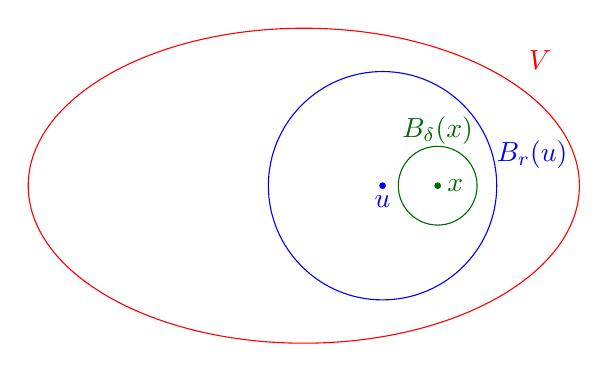
\begin{tikzpicture}
			\draw[red] (0,0) circle [x radius=3.5cm, y radius=2cm] ;
			\draw (3,1.6) node[red]{$V$};
			\draw [blue] (1,0) circle (1.45cm) ;
			\filldraw[blue] (1,0) circle (1pt) node[anchor=north]{$u$};
			\draw (2.9,0.4) node[blue]{$B_r(u)$};
			\draw [green!40!black] (1.7,0) circle (0.5cm) node [yshift=0.7cm]{$B_{\delta}(x)$} ;
			\filldraw[green!40!black] (1.7,0) circle (1pt) node[anchor=west]{$x$};
		\end{tikzpicture}
	\end{center}

	Given $x\in B_r(u)\subset V$, we want $\delta>0$ such that $x\in B_{\delta} (x)\subset B_r(u)\subset V$. Let $d=d(u,x)$. Choose $\delta $ such that $d+\delta<r$ (e.g. $\delta<\frac{r-d}{2}$)

	If $y\in B_{\delta}(x)$ we will be done by showing that $d(u,y)<r$ but $$d(u,y)\leq d(u,x)+d(x,y)<d+\delta<r$$
\end{myproof}

\cor{}{By the result of the proof, we can then show...}
\mlenma{}{Suppose $\vec{v_1}, \dots, \vec{v_n} \in \RR[n]$ is subspace of $\RR^n$.}
\mprop{}{$1 + 1 = 2$.}

\chapter{Algorithms}
\section{Pseudocode}
\begin{algorithm}[H]
	\KwIn{This is some input}
	\KwOut{This is some output}
	\SetAlgoLined
	\SetNoFillComment
	\tcc{This is a comment}
	\vspace{3mm}
	some code here\;
	$x \leftarrow 0$\;
	$y \leftarrow 0$\;
	\uIf{$ x > 5$} {
		x is greater than 5 \tcp*{This is also a comment}
	}
	\Else {
		x is less than or equal to 5\;
	}
	\ForEach{y in 0..5} {
		$y \leftarrow y + 1$\;
	}
	\For{$y$ in $0..5$} {
		$y \leftarrow y - 1$\;
	}
	\While{$x > 5$}tvi {
	$x \leftarrow x - 1$\;
	}
	\Return Return something here\;
	\caption{what}
\end{algorithm}

\chapter{Plots}

\section{3d}

\ex{A 3D plot of $z = 1-x^2-y^2$.}{}

\begin{figure}[!htbp]
	\centering
	\vspace*{10pt}
	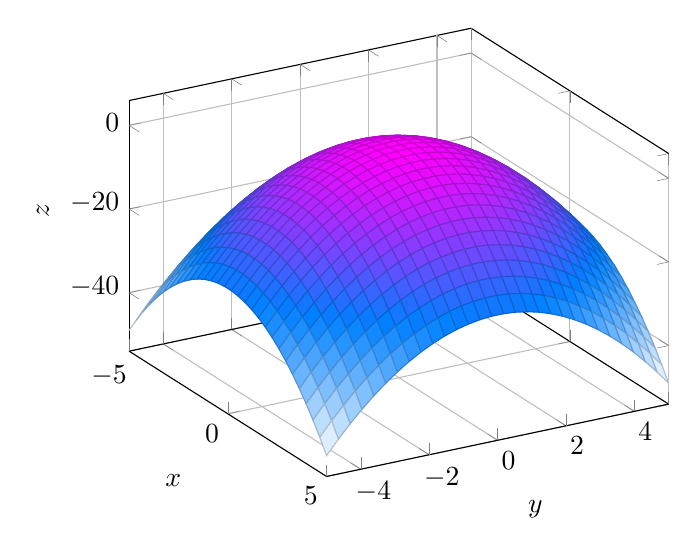
\begin{tikzpicture}
		\begin{axis}[mesh,
				samples=30,
				xlabel={$x$},
				ylabel={$y$},
				zlabel={$z$},
				view={60}{30},
				grid=both,
			]
			\addplot3[
				surf,
				colormap/cool,
				domain=-5:5,
				domain y=-5:5,
			]
			{1-x^2-y^2};
		\end{axis}
	\end{tikzpicture}
	\label{fig:3dplot}
\end{figure}

\chapter{Diagrams}

\section{Circular}

\begin{center}

	\smartdiagramset{custom/.style={
				arrow tip=latex,
				arrow line width=2.5pt,
				module shape=circle,
				font=\footnotesize,
				text width=2cm,
				circular distance=5cm,
				border color=none,
				additions={
						additional item font=\normalsize,
						additional item fill color=lightgray!50,
						additional item offset=1.20cm,
						additional item text width=2.2cm,
						additional item width=5cm
					}
			}
	}


	\smartdiagramset{custom}
	\smartdiagramadd[circular diagram:clockwise]
	{Interlinking / Fusing, Classification / Enrichment,
		Quality Analysis, Evolution / Repair,
		Search / Browsing / Exploration, Extraction,
		Storage / Querying,
		Manual revision / authoring}
	{below of module2/Linked Data Life Cycle}
\end{center}


\end{document}